\section{原型}

\subsection{原型及原型法概述}

\subsubsection{什么是原型}
“原型是一个系统,它内化了一个更迟系统的本质特征。原型系统通常被构造为不完整的系统,以在将来进行改进、补充或者替代。” 

如果在最终的物件产生之前,一个中间物件被用来在一定广度和深度范围内表现这个最终物件,那么这个中间物件就被认为是最终物件在该广度和深度上的原型。 

包括书面描绘、场景叙述、情节串联图板、幻灯演示、动画模拟、屏幕快照和程序代码等在内的各种被用来探索和论证软件系统功能的物件都是软件的原型。

\subsubsection{为什么要使用原型}
\begin{itemize}
    \item 不确定性
    \begin{itemize}
        \item 因为对未来知识有限,而无法确定某种决策的结果
    \end{itemize}
    \item 不确定性是广泛存在的
    \begin{itemize}
        \item 科学的目的是限定、解释不确定性,不是将不确定性转换为确定性
        \item 人们厌恶不确定性:不确定性意味着不完全可控
    \end{itemize}
    \item 软件工程中存在着大量的不确定性,原型、迭代和(方法)验证是人们解决不确定性的主要手段
    \begin{itemize}
        \item 需求的不确定性:需求原型、迭代需求、需求分析技术
        \item 设计的不确定性(设计约束与设计决策):设计原型(体系结构原型)、迭代设计、设计技术
        \item 构造的不确定性(编译错误与运行表现):算法原型、调试、程序语言
        \item 测试的不确定性(缺陷分布):测试环境、测试技术
        \item 管理的不确定性(时间、成本、风险……):管理技术
        \item ……
    \end{itemize}
\end{itemize}

帮助需求工程师及早解决需求的不确定性:
\begin{itemize}
    \item 产品的用户对相关类别的产品没有经验,产品的细节需求存在着不确定性
    \item 用户在完成工作的方式上仍然存在障碍,产品在整体方案的可行性上存在着不确定性
    \item 用户在清晰说明他们的需求方面存在困难,这些相关的需求是有着不确定性的需求
    \item 需求工程师在理解用户的需求上存在困难,在澄清和理解之前,这些需求存在着不确定性
    \item 需求的可行性值得怀疑,即具体需求的可满足性存在着不确定性
    \item 创新性产品,它们的基本需求是潜在的,有着很大的不确定性
\end{itemize}


\subsection{使用原型法进行需求获取}

\subsubsection{基本过程}

\begin{figure}[H]
	\centering
    \vspace{-1em}
	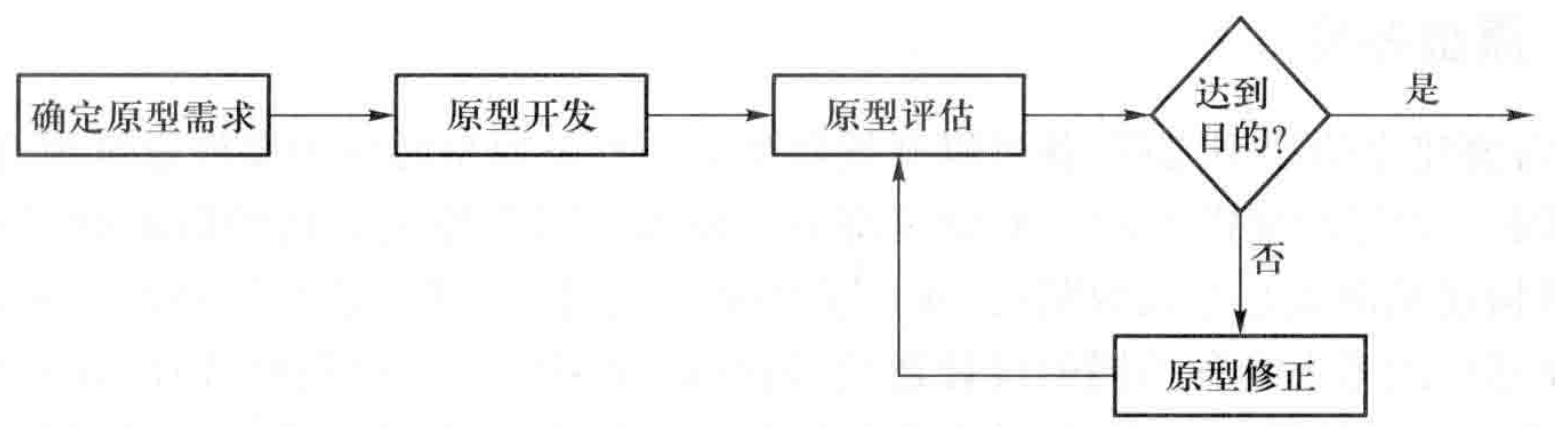
\includegraphics[width=0.65\textwidth]{img/使用原型方法获取需求的典型过程.png}
    \vspace{-1em}
\end{figure}

\subsubsection{确定原型需求}
界定不确定性
\vspace{-0.8em}
\begin{multicols}{3}
    \begin{itemize}
        \item 可能发生的需求变更
        \item 存在冲突的地方
        \item 信息不充分的地方
    \end{itemize}
\end{multicols}
\vspace{-1em}

明确不确定的维度:外观、角色和实现
\begin{itemize}
    \item 外观是指用户对原型物件的具体感觉体验,即用户在使用原型物件时会看到什么、听到什么和感觉到什么 
    \item 角色是指原型物件在用户工作中的价值,也就是说它为什么是对用户有用的
    \begin{itemize}
        \item 原型物件到底能够帮助用户完成什么样的工作
    \end{itemize}
    \item 实现是指原型物件完成功能的细节技术和方法 
\end{itemize}

\subsubsection{原型开发}
开发原型时的主要注意事项有以下几点
\vspace{-0.8em}
\begin{multicols}{2}
    \begin{itemize}
        \item 将探索不确定功能需求的原型构建得易修改
        \item 让探索可行性的原型收集充分的数据
        \item 控制开发成本
    \end{itemize}
\end{multicols}
\vspace{-1em}

\subsubsection{原型评估}
\begin{itemize}
    \item 需要获取的评估者反馈
    \vspace{-0.8em}
    \begin{multicols}{3}
    \begin{itemize}
        \item 评估者反应
        \item 评估者建议
        \item 创新思想
    \end{itemize}
    \end{multicols}
    \vspace{-1em}
    \item 可以创建一些脚本来指导评估者的体验活动 
    \item 务必要让合适的人从恰当的角度来评估原型
    \item 观察评估人员使用原型的过程
    \item 创造一个无偏见的环境,让评估人员畅所欲言
\end{itemize}

\subsubsection{原型修正}
原型修正一方面要依据评估人员的反馈, 另一方面也要考虑事先的原型调整计划。原型一定要开发的容易修改。


\subsection{抛弃式原型与演化式原型}
按照[Floyd 1984]的分类,可以将原型开发方法分为3种类型
\begin{itemize}
    \item 探索式(exploratory)
    \begin{itemize}
        \item 以缺陷需求开始继而不断调整和修正需求的原型开发方式称为探索式,要尽可能的调整各种设计选项
        \item 演示原型,严格意义上的原型
    \end{itemize}
    \item 实验式(experimental)
    \begin{itemize}
        \item 以清晰的用户需求和模糊的实现方法、实现效果、可行性开始,明确需求的可行性和技术实现方案
        \item 定义一个对原型的评估方法,确定评估的属性
        \item 试验原型
    \end{itemize}
    \item 演化式(evolutionary)
    \begin{itemize}
        \item 以清晰的原型化需求和项目积累下来的原型资产为开始
        \item 原型化的需求,也有项目积累下来的原型资产 
        \item 引示系统原型
    \end{itemize}
\end{itemize}

% 设定尺寸单位
\setlength{\TPHorizModule}{\textwidth}
\setlength{\TPVertModule}{\textwidth}
 
% 排版文本框
\begin{textblock}{0.5}(0.775,1.35)
{\fangsong
\begin{compactitem}
    \item 演示原型
    \begin{compactitem}
        \item 主要被用在启动项目阶段 
        \item 目的让用户相信应用系统的开发是可行的 
    \end{compactitem}
    \item 严格意义上的原型
    \begin{compactitem}
        \item 主要被用在分析需求阶段 
        \item 用来阐明用户界面或者系统功能的某些特定方面 
    \end{compactitem}
    \item 试验原型
    \begin{compactitem}
        \item 主要被用在构建系统阶段 
        \item 帮助开发者澄清他们所面对的一些和系统构建相关的技术问题 
    \end{compactitem}
    \item  引示系统原型
    \begin{compactitem}
        \item 会被开发在系统开发的各个阶段 
        \item 用作最终系统的构建核心 
    \end{compactitem}
\end{compactitem}}
\end{textblock}

  
探索式和实验式方法产生的原型产品又被称为抛弃式原型 
\begin{itemize}
    \item 花费最小的代价,争取最快的速度 
    \item 可能会使用简易的开发工具和不成熟的构造技术 
    \item 可能会忽略或简化处理原型目的不相关的功能特征 
    \item 要\textbf{坚决抛弃抛弃式原型}
\end{itemize}

演化式原型方法产生的原型产品被称为演化式原型
\begin{itemize}
    \item 质量要从一开始就能达到最终系统的要求 
    \item 要易于进行扩展和频繁改进,因此开发者必须重视演化式原型的设计 
    \item 仅应该被用于处理清晰的需求、规格说明和技术方案 
\end{itemize}

\subsection{控制原型开发成本}

\subsubsection{依据抛弃式特征控制原型成本}
因为基于不确定的需求基础,所以抛弃式原型难免反复修改,导致代码质量较低,应该坚决抛弃。

抛弃式原型的贡献不在于它的代码,而是它所包含的内容,它说明了正确的需求和正确的技术方案,如果认识不到这一点,他们就只能得到低质量的代码,而丢失真正宝贵的内容。

控制抛弃式原型的成本
\begin{itemize}
    \item “不要过于详细地构建抛弃式原型,只要它能够满足原型制作的目标就足够了。要抵制住诱惑,也要顶住用户的压力,不要向抛弃式原型添加更多的功能。”[Wiegers2003]
\end{itemize}

\subsubsection{控制水平原型的开发成本}
\vspace{-0.8em}
\begin{multicols}{2}
    \begin{itemize}
        \item 水平原型方法
        \begin{itemize}
            \item 它仅仅实现选定功能所有层次中的某些特定层次 
            \item 建立的原型产品称为水平原型
            \item 要把注意力集中在概括性需求和工作流问题上 
        \end{itemize}
        \item 垂直原型方法
        \begin{itemize}
            \item 它会触及到选定功能实现的所有层次
            \item 建立的原型产品称为垂直原型
            \item 要保证真实实现它的各种功能
        \end{itemize}
        \item 用尽可能低的成本开发水平原型
    \end{itemize}
\end{multicols}
\vspace{-1em}

\subsubsection{用尽量简单的介质降低成本}
\begin{figure}[H]
	\centering
    \vspace{-1em}
	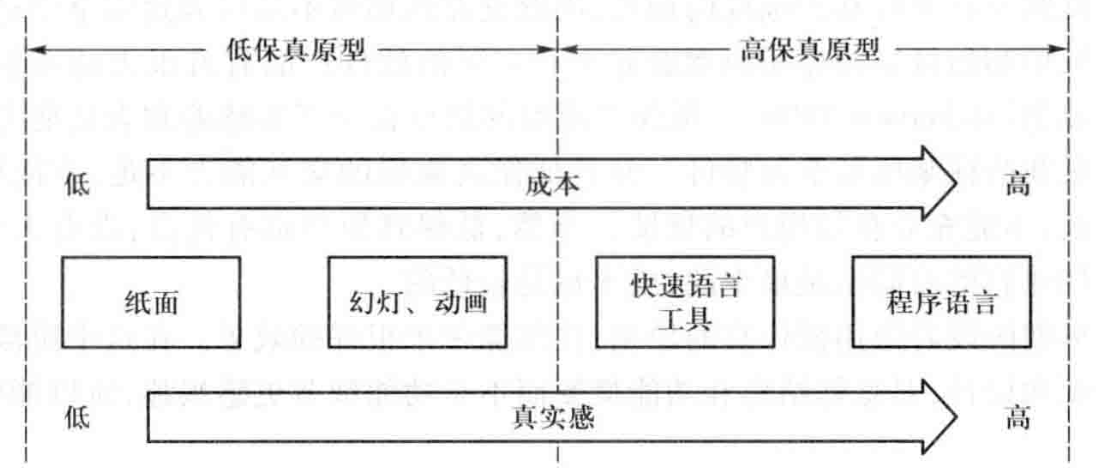
\includegraphics[width=0.65\textwidth]{img/原型的常见介质.png}
    \caption*{原型的常见介质}
    \vspace{-1em}
\end{figure}

\subsection{善用故事板原型}
\begin{figure}[H]
	\centering
    \vspace{-1em}
	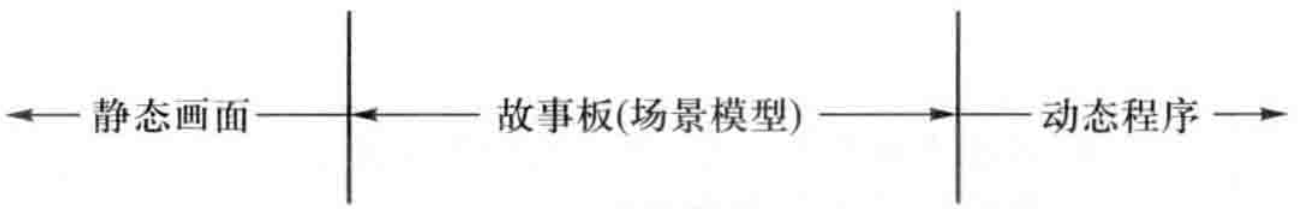
\includegraphics[width=0.6\textwidth]{img/故事板原型.png}
    \vspace{-1em}
\end{figure}

故事板最早是好莱坞在设计电影场景和卡通故事时使用的,卡通制作者通过勾画出一系列相连的图片来展示一个卡通故事,具有更直观、可视化的故事叙述能力

将原来分散的功能与步骤组织成故事,让普通人能够更好地体验与评估

原型和用例/场景通常结合使用[Mannio 2001]:为需要探索和澄清的用例/场景建立故事板原型,或者依据故事板原型的评估结果建立清晰、明确的用例/场景描述

\begin{figure}[H]
	\centering
    \vspace{-1em}
	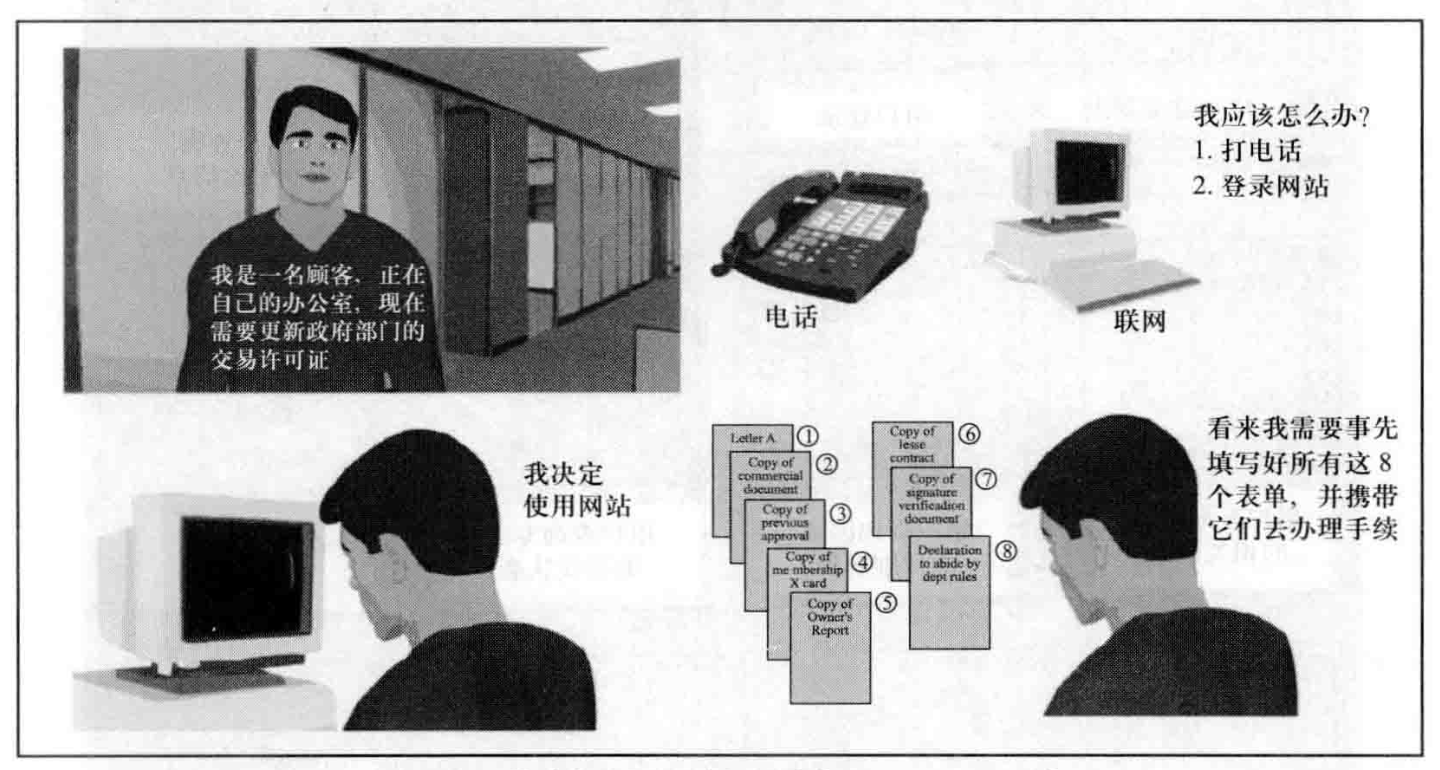
\includegraphics[width=0.75\textwidth]{img/故事板原型示例.png}
    \caption*{故事板原型示例}
    \vspace{-1em}
\end{figure}

故事板原型构建
\begin{itemize}
    \item 明确故事板原型要素
    \vspace{-0.8em}
    \begin{multicols}{3}
    \begin{itemize}
        \item 角色(Who)
        \item 内容(What)
        \item 方法(How)
    \end{itemize}
    \end{multicols}
    \vspace{-1em}
    \item 建不同类型的故事板原型
    \begin{itemize}
        \item 被动(Passive)故事板原型$\rightarrow$连环画
        \item 主动(Active)故事板原型$\rightarrow$漫画
        \item 交互(Interactive)故事板原型$\rightarrow$网页   
    \end{itemize}
\end{itemize}

\begin{figure}[H]
	\centering
    \vspace{-0.5em}
	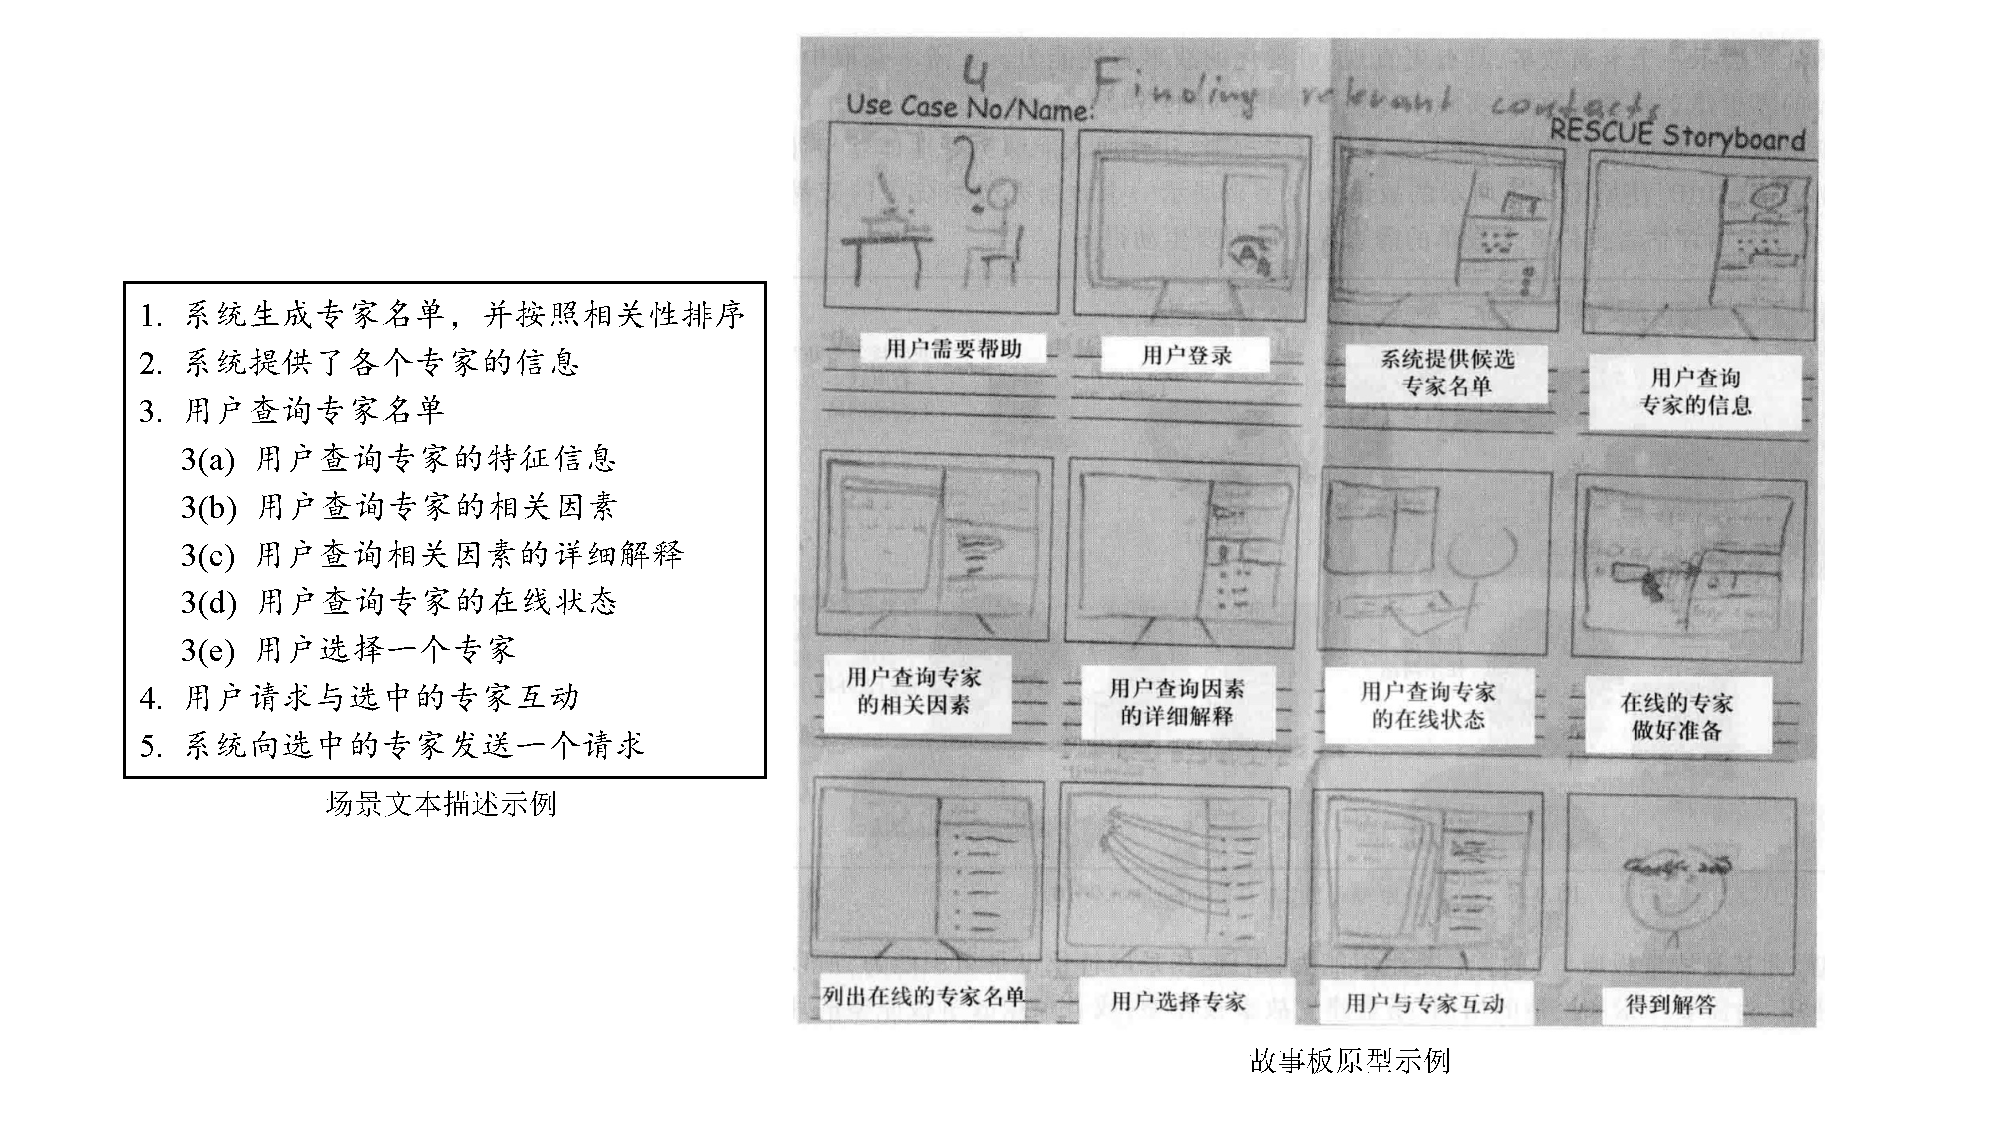
\includegraphics[width=0.83\textwidth]{img/为场景描述建立更直观的故事板原型.pdf}
    \caption*{为场景描述建立更直观的故事板原型}
    \vspace{-1em}
\end{figure}

\subsection{原型方法的风险}
\begin{itemize}
    \item 原型开发工作投入太多的工作,使得开发团队消耗了过多的时间和过大的成本
    \item 涉众看到了一个正在运行的原型,得出产品几乎已经完成的结论,从而提出快速交付产品的不当要求
    \begin{itemize}
        \item 不要将原型的功能开发的太好,以免用户提出“交付”的要求
    \end{itemize}
    \item 用户可能会被原型所表现出来的非功能特性遮蔽了眼睛,从而忽略了他们更应该重视的功能特性
    \item 在澄清需求不确定性的同时也可能会掩盖一些用户的假设,这些假设将会无从发现
\end{itemize}

\subsection{总结}
\begin{itemize}
    \item 原型是软件开发当中消除不确定性风险的有效工具,是一种有效的需求获取方法
    \item 原型的体系是复杂的,不同类型的原型具有不同的作用和创建要求,实践当中应该综合考虑各种应用因素选择合适的类别
    \item 一个完整的原型方法过程可以帮助更有效的应用原型方法
    \item 原型方法的应用可能会给项目带来相应的风险,需要妥善的加以解决
\end{itemize}
